\documentclass[journal,12pt,twocolumn]{IEEEtran}

\usepackage{enumitem}
\usepackage{amsmath}
\usepackage{amssymb}
\usepackage{gensymb}
\usepackage{graphicx}
\usepackage{txfonts}         
\usepackage{listings}
\usepackage{lstautogobble}
\usepackage{mathtools}
\usepackage{bm}
\usepackage{hyperref}

\newcommand{\solution}{\noindent \textbf{Solution: }}
\providecommand{\pr}[1]{\ensuremath{\Pr\left(#1\right)}}
\providecommand{\brak}[1]{\ensuremath{\left(#1\right)}}
\providecommand{\cbrak}[1]{\ensuremath{\left\{#1\right\}}}
\providecommand{\sbrak}[1]{\ensuremath{\left[#1\right]}}
\providecommand{\mean}[1]{E\left[ #1 \right]}
\providecommand{\var}[1]{\mathrm{Var}\left[ #1 \right]}
\providecommand{\der}[1]{\mathrm{d} #1}
\providecommand{\gauss}[2]{\mathcal{N}\ensuremath{\left(#1,#2\right)}}
\providecommand{\mbf}{\mathbf}
\providecommand{\abs}[1]{\left\vert#1\right\vert}
\providecommand{\norm}[1]{\left\lVert#1\right\rVert}
\providecommand{\z}[1]{{\mathcal{Z}}\{#1\}}
\providecommand{\ztrans}{\overset{\mathcal{Z}}{ \rightleftharpoons}}

\providecommand{\parder}[2]{\frac{\partial}{\partial #2} \brak{#1}}

\let\StandardTheFigure\thefigure
\let\vec\mathbf

\numberwithin{equation}{section}
\renewcommand{\thefigure}{\theenumi}
\renewcommand\thesection{\arabic{section}}

\newcommand{\myvec}[1]{\ensuremath{\begin{pmatrix}#1\end{pmatrix}}}
\newcommand{\mydet}[1]{\ensuremath{\begin{vmatrix}#1\end{vmatrix}}}

\DeclareMathOperator*{\argmin}{arg\,min}
\DeclareMathOperator*{\argmax}{arg\,max}

\lstset {
	frame=single, 
	breaklines=true,
	columns=fullflexible,
	autogobble=true
}             
                               
\title{Digital Signal Processing \\ \Large EE3900: Linear Systems and Signal Processing \\ \large Indian Institute of Technology Hyderabad}
\author{Ankit Saha \\ \normalsize AI21BTECH11004 \\ \vspace*{20pt} \normalsize 1 Aug 2022}


\begin{document}

	\maketitle
	
	\section{Software Installation}
	Install the necessary packages by running the following commands
	\begin{lstlisting}
		sudo dnf up
		sudo dnf install libffi-dev libsndfile1 python3-scipy  python3-numpy python3-matplotlib 
		pip install cffi pysoundfile 
	\end{lstlisting}

	\section{Digital Filter}
	\begin{enumerate}[label=\thesection.\arabic*,ref=\thesection.\theenumi]
	\item \label{prob:input} Download the sound file from  
	\begin{lstlisting}
		wget https://github.com/Ankit-Saha-2003/EE3900/raw/main/Assignment_1/codes/Sound_Noise.wav
	\end{lstlisting}
	
	\item \label{prob:spectrogram} You will find a spectrogram at \href{https://academo.org/demos/spectrum-analyzer}{\url{https://academo.org/demos/spectrum-analyzer}}. Upload the sound file that you downloaded in Problem \ref{prob:input} in the spectrogram  and play.  Observe the spectrogram. What do you find?
	
	\solution There is a lot of background noise and the key strokes are audible. This noise is represented by the large blue and red regions spread from 440 Hz to beyond 18.9 kHz. The key tones are represented by the yellow lines that are present in the lower regions between 440 Hz and 5.1 kHz.
	
	\item \label{prob:output} Write the python code for removal of out of band noise and execute the code. 
	
	\solution Download the python code for the reduction of noise by executing the following command
	\begin{lstlisting}
		wget https://github.com/Ankit-Saha-2003/EE3900/raw/main/Assignment_1/codes/2.3.py
	\end{lstlisting}
	
	Run the code by executing
	\begin{lstlisting}
		python 2.3.py
	\end{lstlisting}
	
	Play the newly created audio file by executing
	\begin{lstlisting}
		aplay Sound_With_Reduced_Noise.wav
	\end{lstlisting}
	
	\item The output of the python script in Problem \ref{prob:output} is the audio file Sound\_With\_Reduced\_Noise.wav. Play the file in the spectrogram in Problem \ref{prob:spectrogram}. What do you observe?
	
	\solution The noise has been reduced considerably and the key strokes are not audible anymore. The blue region is restricted between 440 Hz and 5.1 kHz and there are no signals beyond this range.
	
	
	\end{enumerate}
	
	\section{Difference Equation}
	\begin{enumerate}[label=\thesection.\arabic*,ref=\thesection.\theenumi]
	\item Let
	\begin{equation}
		x(n) = \cbrak{\underset{\uparrow}{1},2,3,4,2,1}
	\end{equation}
	Sketch $x(n)$
	\item Let
	\begin{multline}
		\label{eq:iir_filter}
		y(n) + \frac{1}{2}y(n-1) = x(n) + x(n-2), \\
 		y(n) = 0, n < 0
	\end{multline}
	
	Sketch $y(n)$

	\solution Download the following Python code that plots Fig. \ref{fig-3.2}.
	\begin{lstlisting}
		wget https://github.com/Ankit-Saha-2003/EE3900/raw/main/Assignment_1/codes/3.2.py
	\end{lstlisting}
	
	Run the code by executing
	\begin{lstlisting}
		python 3.2.py
	\end{lstlisting}

	\begin{figure}[!ht]
		\centering
		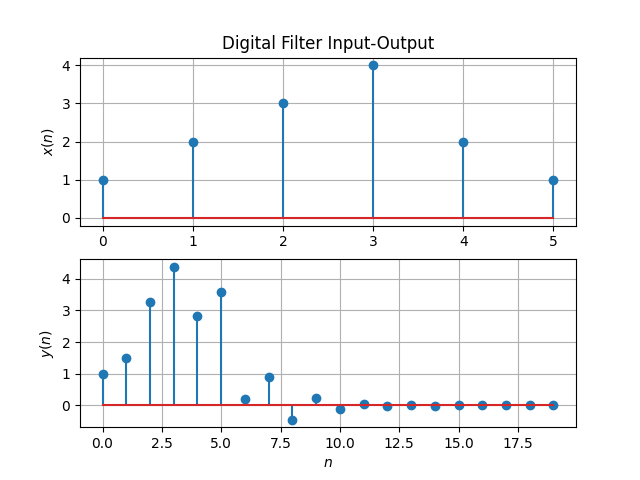
\includegraphics[width=\columnwidth]{./figs/3.2.png}
		\caption{The sketches of $x(n)$ and $y(n)$}
		\label{fig-3.2}	
	\end{figure}
	\end{enumerate}
	
	\section{$Z$-transform}
	\begin{enumerate}[label=\thesection.\arabic*]
	\item The $Z$-transform of $x(n)$ is defined as
	\begin{equation}
		\label{eq:z_trans}
		X(z)={\mathcal {Z}}\{x(n)\}=\sum _{n=-\infty }^{\infty }x(n)z^{-n}
	\end{equation}
	Show that
	\begin{equation}
		\label{eq:shift1}
		{\mathcal {Z}}\{x(n-1)\} = z^{-1}X(z)
	\end{equation}
	and find
	\begin{equation}
		{\mathcal {Z}}\{x(n-k)\} 
	\end{equation}
	
	\solution 
	\begin{align}
		{\mathcal {Z}}\{x(n-1)\} &= \sum _{n=-\infty }^{\infty }x(n - 1)z^{-n} 
	\end{align}
	
	Substitute $n - 1 = m$
	\begin{align}
		{\mathcal {Z}}\{x(n-1)\} &=  \sum _{m=-\infty }^{\infty }x(m)z^{-(m+1)} \\
		&= z^{-1} \sum _{m=-\infty }^{\infty }x(m)z^{-m} \\
		&= z^{-1} {\mathcal {Z}}\{x(m)\} \\	
		&= z^{-1} X(z) \\
		{\mathcal {Z}}\{x(n-k)\} &=  \sum _{n=-\infty }^{\infty }x(n - k)z^{-n} \\
		&=  \sum _{m=-\infty }^{\infty }x(m)z^{-(m+k)} \\
		&= z^{-k} \sum _{m=-\infty }^{\infty }x(m)z^{-m} \\
		&= z^{-k} X(z)
	\end{align}	
	
	\item Find
	\begin{equation}
		H(z) = \frac{Y(z)}{X(z)}
	\end{equation}

	from  \eqref{eq:iir_filter} assuming that the $Z$-transform is a linear operation.

	\solution 
	\begin{align}
		y(n) + \frac{1}{2}y(n-1) = x(n) + x(n-2)
	\end{align}
	
	On applying the $Z$-transform on both sides of the equation, we get
	\begin{align}
		{\mathcal {Z}}\cbrak{y(n) + \frac{1}{2}y(n-1)} = {\mathcal {Z}}\{x(n) + x(n-2)\}
	\end{align}
	
	Since we are assuming that the $Z$-transform is a linear operation,
	\begin{align}
		\z{y(n)} + \frac12 \z{y(n-1)} &= \z{x(n)} + \z{x(n-2)} \\
		\implies Y(z) + \frac12 z^{-1} Y(z) &= X(z) + z^{-2} X(z) \\
		\implies Y(z) \brak{1 + \frac12 z^{-1}} &= X(z) (1 + z^{-2}) \\
		\therefore H(z) = \frac{Y(z)}{X(z)} &= \frac{1 + z^{-2}}{1 + \frac12 z^{-1}}
	\end{align}
	
	\item Find the Z transform of 
	\begin{equation}
		\delta(n) =
		\begin{cases}
			1 & n = 0 \\
			0 & \text{otherwise}
		\end{cases}
	\end{equation}
	and show that the $Z$-transform of
	\begin{equation}
	\label{eq:unit_step}
	u(n) =
	\begin{cases}
		1 & n \ge 0 \\
		0 & \text{otherwise}	
	\end{cases}
	\end{equation}
	is
	\begin{equation}
		U(z) = \frac{1}{1-z^{-1}} \quad \abs{z} > 1
	\end{equation}
	
	\solution 
	\begin{align}
		\z{\delta(n)} &= \sum _{n=-\infty }^{\infty }\delta(n)z^{-n} \\
		&= \delta(0) z^{-0} \\
		&= 1 
	\end{align}
	\begin{align}
		\z{u(n)} &= \sum _{n=-\infty }^{\infty } u(n)z^{-n} \\
		&= \sum _{n=0}^{\infty } \brak{z^{-1}}^n 
	\end{align}
	
	This is the sum of an infinite geometric progression with first term $1$ and common ratio $z^{-1}$. The sum converges when
	\begin{equation}
		\abs{z^{-1}} < 1 \iff \abs{z} > 1
	\end{equation}
	
	Therefore,
	\begin{equation}
		U(z) = \z{u(n)} = \frac{1}{1 - z^{-1}} \quad \abs{z} > 1
	\end{equation}

	\item Show that 
	\begin{equation}
		\label{eq:anun}
		a^nu(n) \ztrans \frac{1}{1-az^{-1}} \quad \abs{z} > \abs{a}
	\end{equation}
	
	\solution
	\begin{align}
		\z{a^nu(n)} &= \sum _{n=-\infty }^{\infty } a^nu(n)z^{-n} \\
		&= \sum _{n=0}^{\infty } \brak{az^{-1}}^{n} 
	\end{align}
	
	This is the sum of an infinite geometric progression with first term $1$ and common ratio $az^{-1}$. The sum converges when
	\begin{equation}
		\abs{az^{-1}} < 1 \iff \abs{z} > \abs{a}
	\end{equation}
	
	Therefore,
	\begin{equation}
		\z{a^nu(n)} = \frac{1}{1-az^{-1}} \quad \abs{z} > \abs{a}
	\end{equation}
	
	\item Let
	\begin{equation}
		H\brak{e^{\j \omega}} = H\brak{z = e^{\j \omega}}.
	\end{equation}
	Plot $\abs{H\brak{e^{\j \omega}}}$.  Comment.  $H(e^{\j \omega})$ is known as the {\em Discret Time Fourier Transform} (DTFT) of $x(n)$
	
	\solution

	
	\end{enumerate}
	
	
\end{document}